\section{Introduction}

% Causality: statistical + symbolic AI
\begin{frame}
    \frametitle{Artificial Intelligence}
    \begin{itemize}
        \item Statistical Artificial Intelligence
            \begin{itemize}
                \item Deduction
                \item Data
                \item Opaque
            \end{itemize}
        \item Symbolic Artificial Intelligence
            \begin{itemize}
                \item Induction
                \item Knowledge
                \item Interpretable
            \end{itemize}
    \end{itemize}
\end{frame}

\begin{frame}
    \frametitle{Statistical Artificial Intelligence}
    
    \only<1>{
        \twoimg{1introduction/stat1.png}{1introduction/stat1appl.jpg}
    }
    \only<2>{
        \twoimg{1introduction/stat2.png}{1introduction/stat2appl.jpeg}
    }
    \only<3>{
        \twoimg{1introduction/stat3.jpeg}{1introduction/stat3appl.png}
    }
    \only<4>{
        \begin{center}
            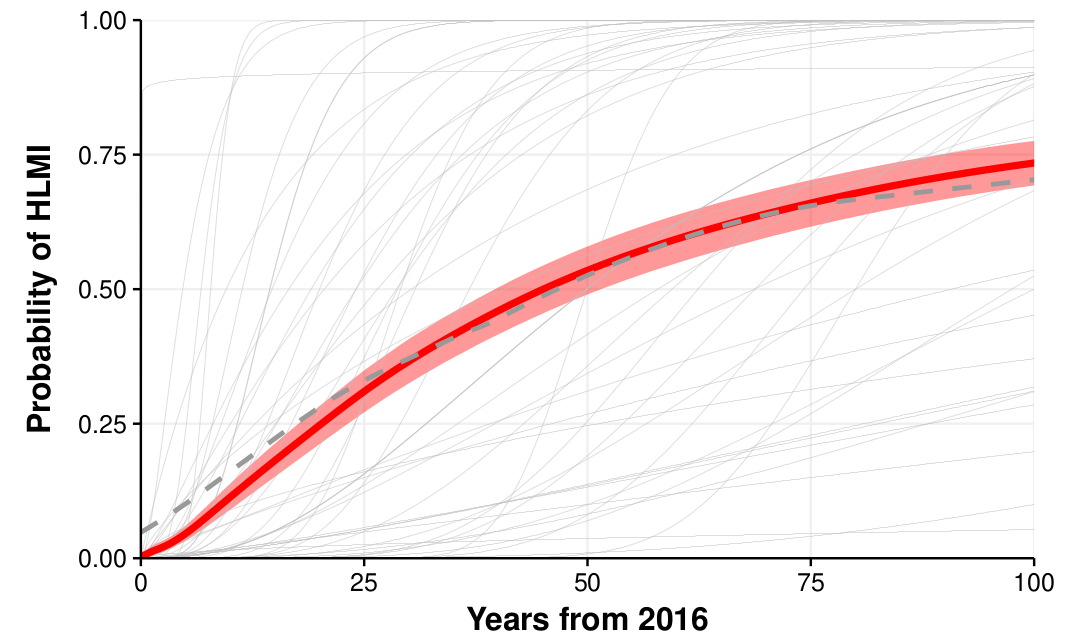
\includegraphics[width=.8\textwidth]{1introduction/hlmi.png}
        \end{center}
    }
\end{frame}

\begin{frame}
    \frametitle{Symbolic AI}
    
    \only<1>{
        \twoimg{1introduction/symb1}{1introduction/symb1appl}
    }
    \only<2>{
        \twoimg{1introduction/symb2}{1introduction/symb2appl}
    }
    \only<3>{
        \twoimg{1introduction/symb3}{1introduction/symb3appl}
    }
\end{frame}

% Questions answerable with causality (encoding causal assumptions)
\begin{frame}
    \frametitle{Causality}

    \only<1>{
        \twoimg{1introduction/joint_distr}{1introduction/rct}
    }

    \only<2-3>{
        \begin{columns}
            \begin{column}{0.4\textwidth}
                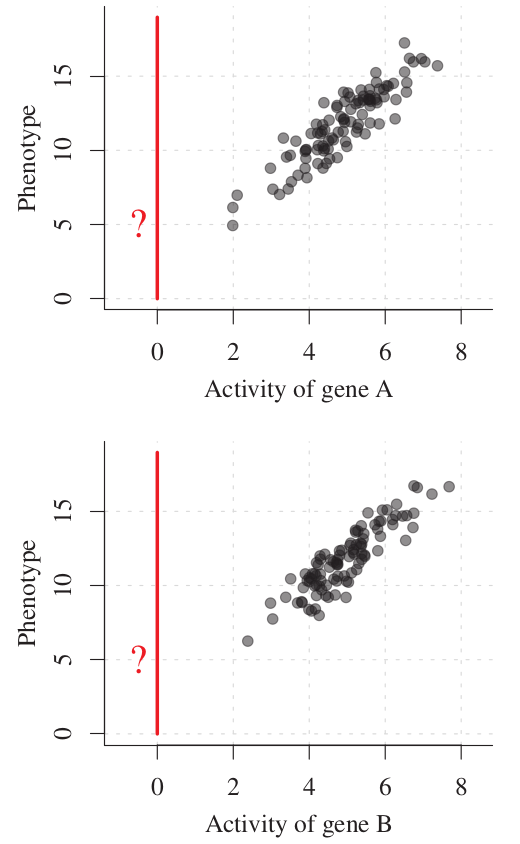
\includegraphics[width=\textwidth]{1introduction/causalknowledgeA.png}
            \end{column}
            \begin{column}{0.4\textwidth}
                \includegraphics<3>[width=\textwidth]{1introduction/causalknowledgeB.png}
            \end{column}
        \end{columns}
    }

    \only<4>{
        \begin{center}
            \Large Reichenbach's Common Cause Principle

            \vspace{10mm}

            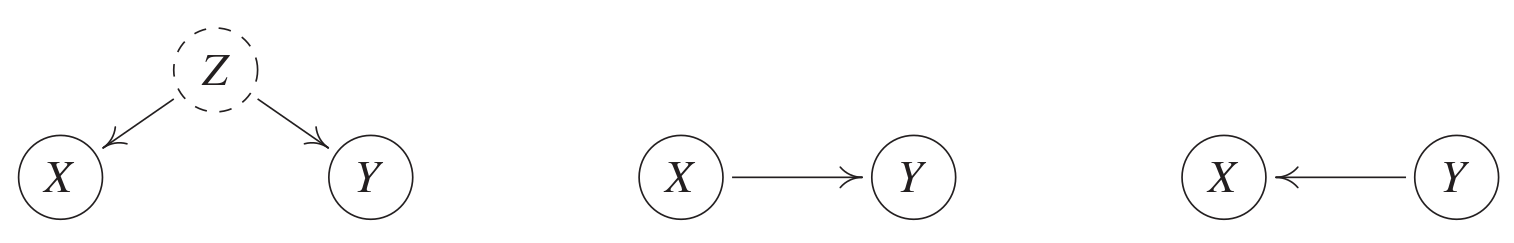
\includegraphics[width=\textwidth]{1introduction/reichenback.png}
        \end{center}
    }

    % Questions answerable by causality
    \only<5>{
        \begin{center}
            {\huge $\Prb(X=x|Y=y)$} 

            \vspace{10mm}
            
            "What is the chance that I am infected with Covid ($X=x$), \\
            given that I live in Utrecht ($Y=y$)?"
        \end{center}
    }

    \only<6>{
        \begin{center}
            {\huge $\Prb(X=x|do(Y=y),Z=z)$} 

            \vspace{10mm}
            
            "What will happen to the number of cases per capita ($X=x$) \\
            in Delft ($Z=z$) \\
            if we introduce a lock-down ($do(Y=y)$)?"
        \end{center}
    }

    \only<7>{
        \begin{center}
            {\huge $\Prb(y_x|x',y',do(Z=z),W=w)$} 

            \vspace{10mm}
            
            "What is the chance that I would have been infected with Covid, if I had not worn a face mask in the train yesterday ($y_x$)? \\
            I know that I actually did wear the mask ($x'$) \\
            and that I am not infected ($y'$). \\
            The train went to Bovenkarspel ($W=w$) \\
            and all other people wore a mask because the government made it mandatory ($do(Z=z)$)."
        \end{center}
    }



\end{frame}




% Modeling causality: SCMs to encode causal assumptions (focus?: math or methods)


\begin{frame}
    \frametitle{Structural Causal Model}
    
    \only<1>{
        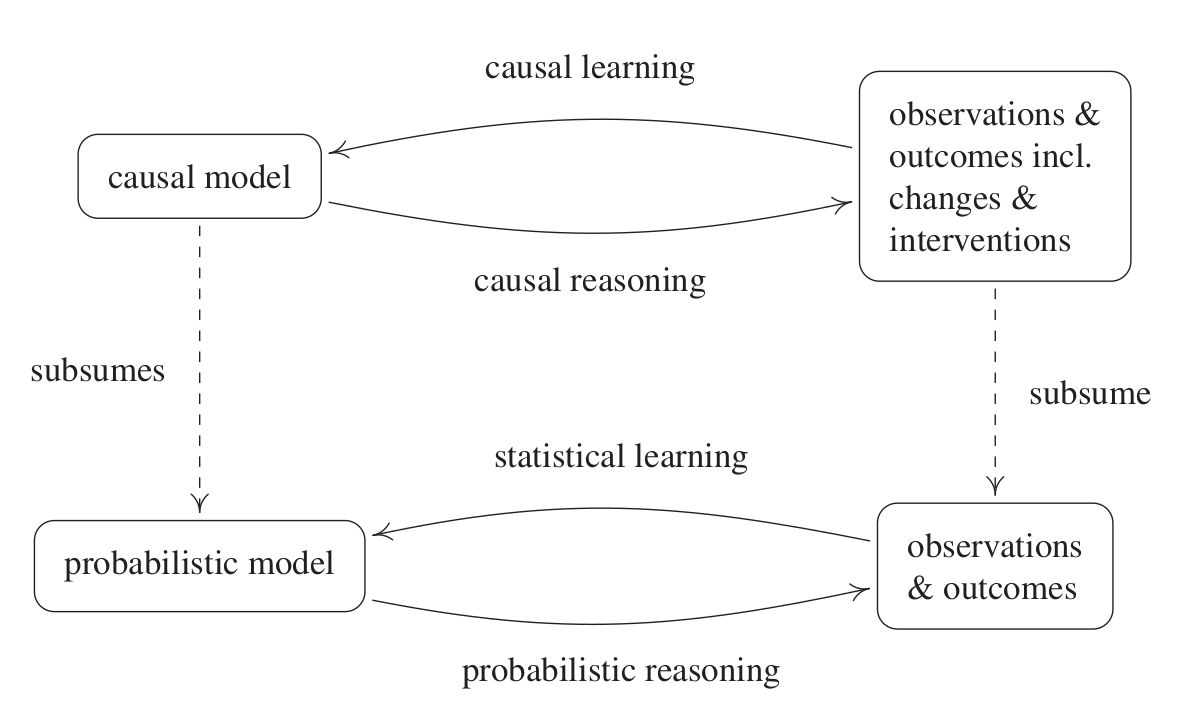
\includegraphics[width=\textwidth]{1introduction/causality_stats.png}
    }

    \only<2>{
        \begin{center}
            \huge $$\C{M}: \begin{cases}
                X_i &= f_i(\B{X}_{\pasub{}{i} \cap \C{I}}, \B{E}_{\pasub{}{i} \cap \C{J}}) \\
                p_{\B{E}} & = \prod_{j\in\C{J}} p_{E_j}
            \end{cases}$$
        \end{center}

        \vspace{5mm}

        $\C{M}$: structural causal model

        $\B{X}$: endogenous variables

        $\B{E}$: exogenous variables
    }

    \only<3>{
        \begin{center}
            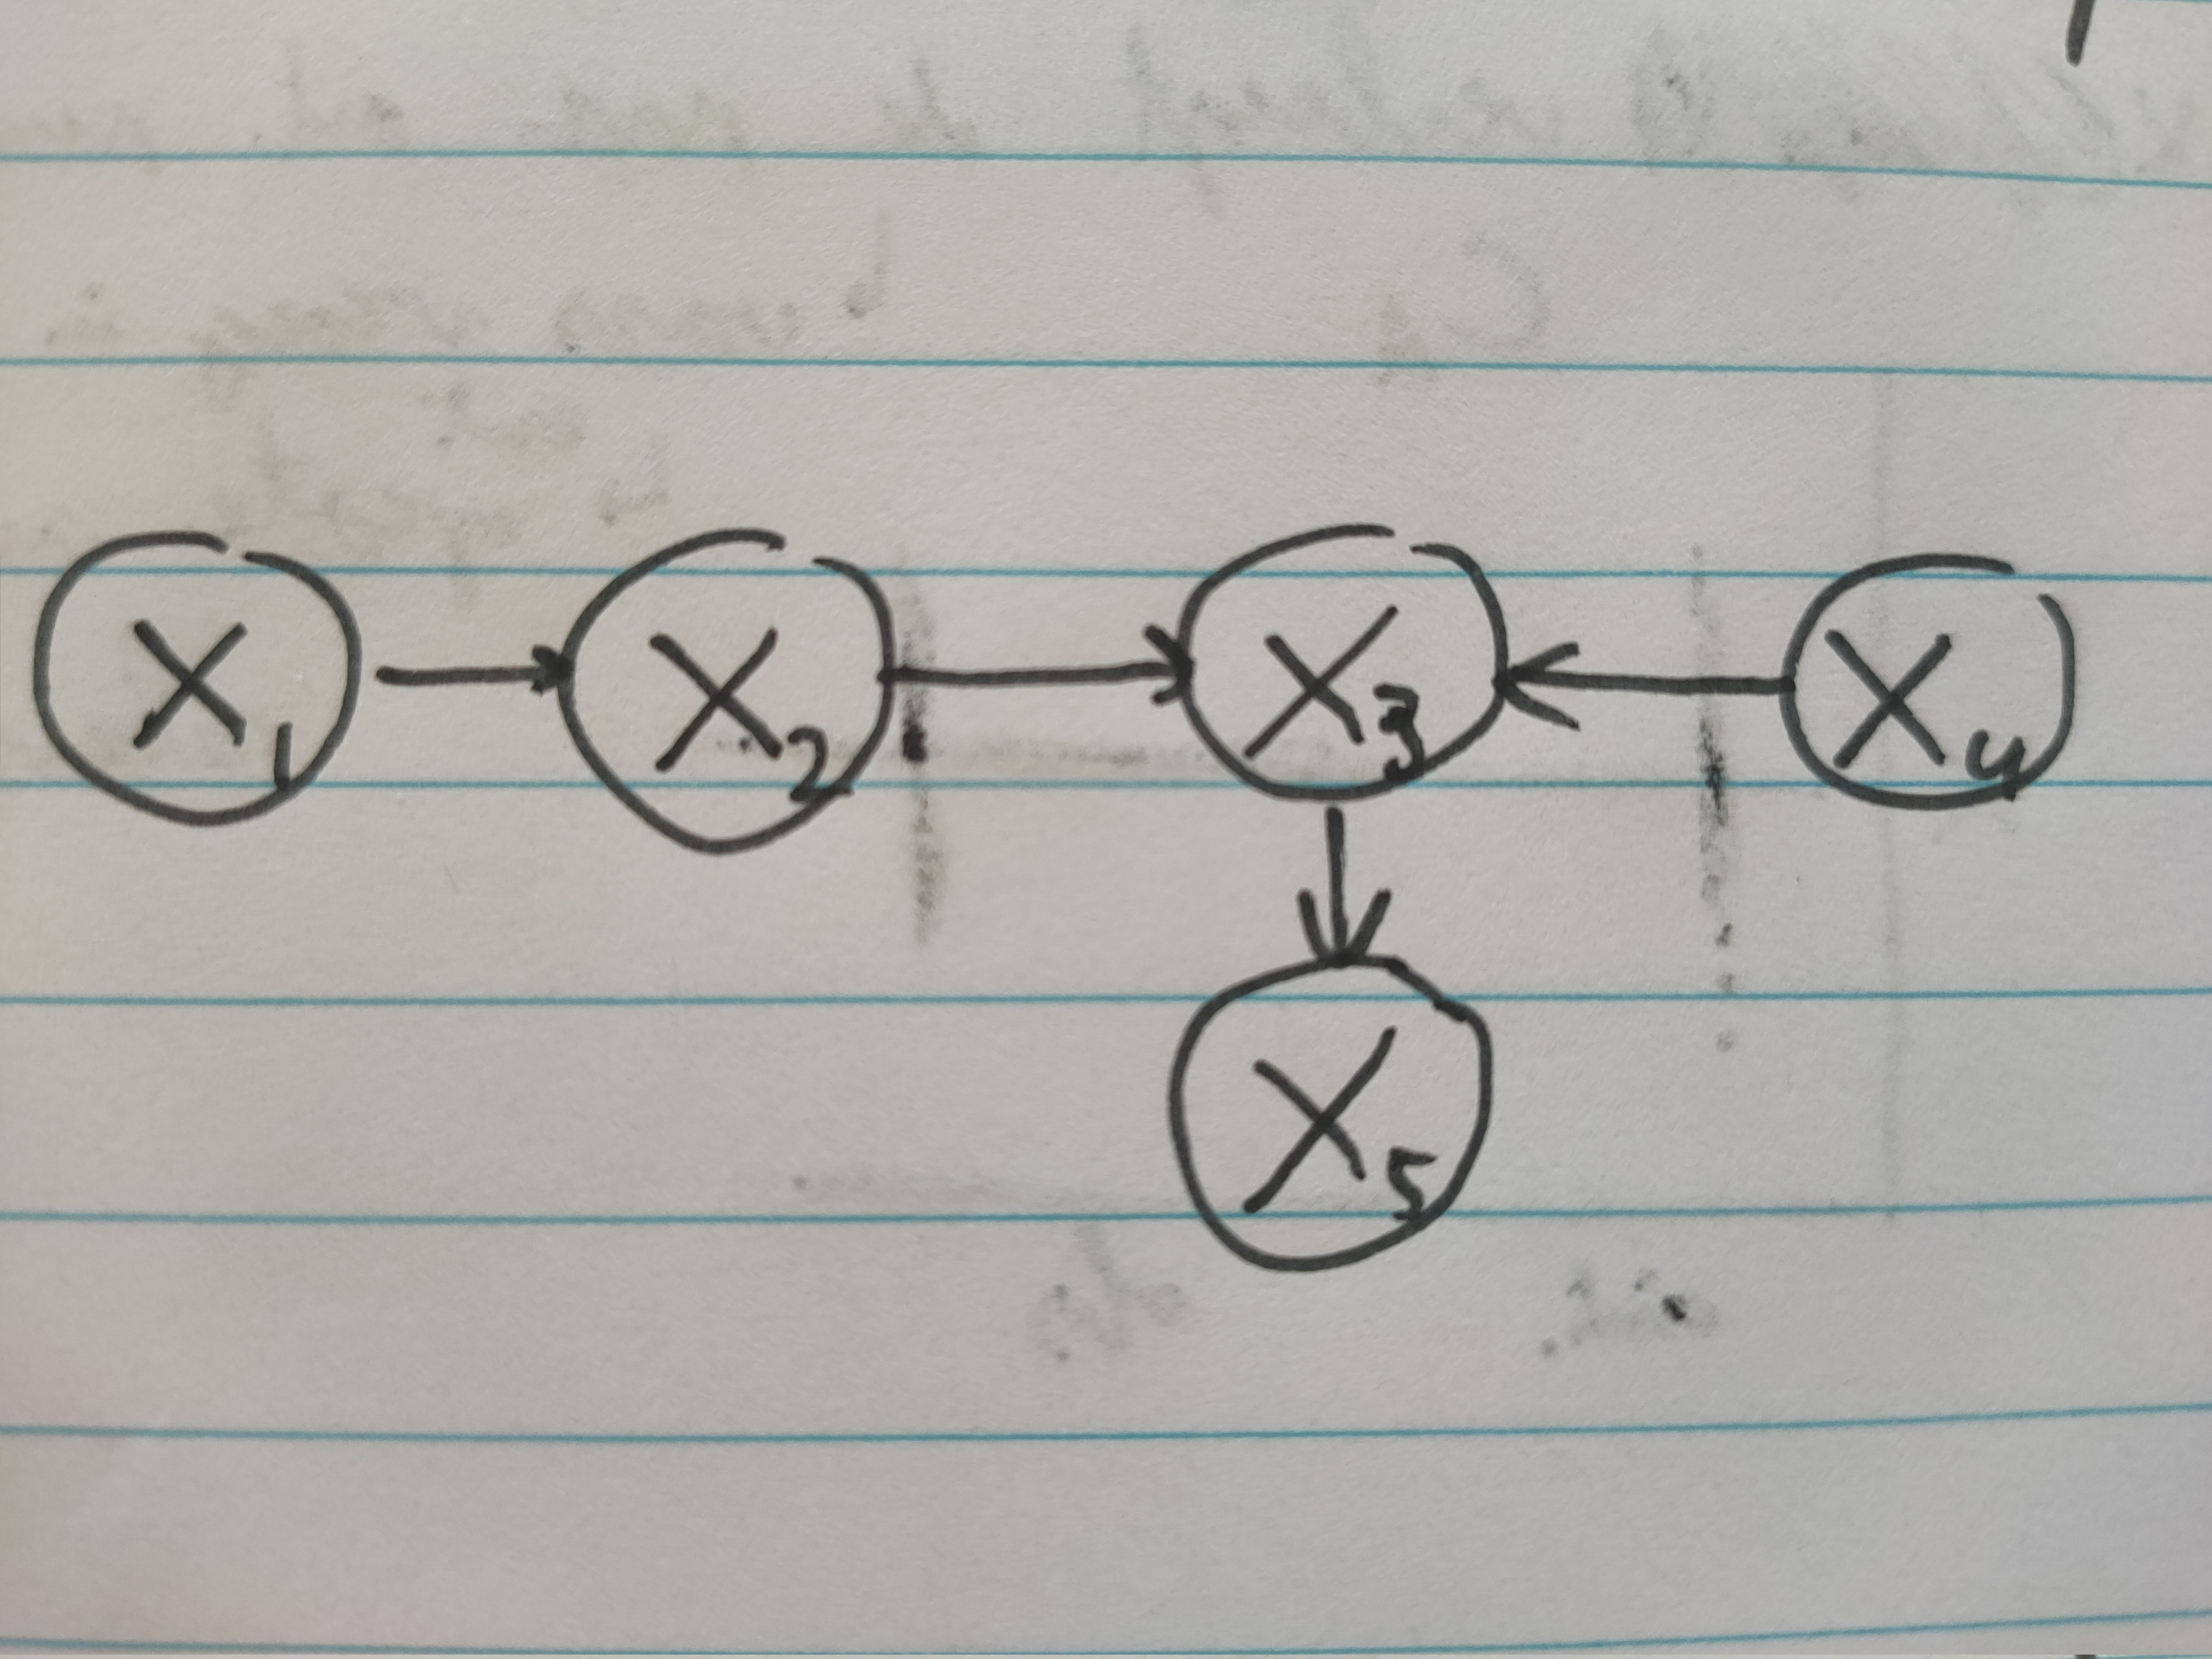
\includegraphics[width=\textwidth]{paper/2dsep}

            \huge $$\dsep{\B{A}}{\B{B}}{\B{C}}{\C{G}} \implies \indep{\B{A}}{\B{B}}{\B{C}}{\Prb_{\B{X}}}$$
        \end{center}
    }

    \only<4>{
        \begin{center}
            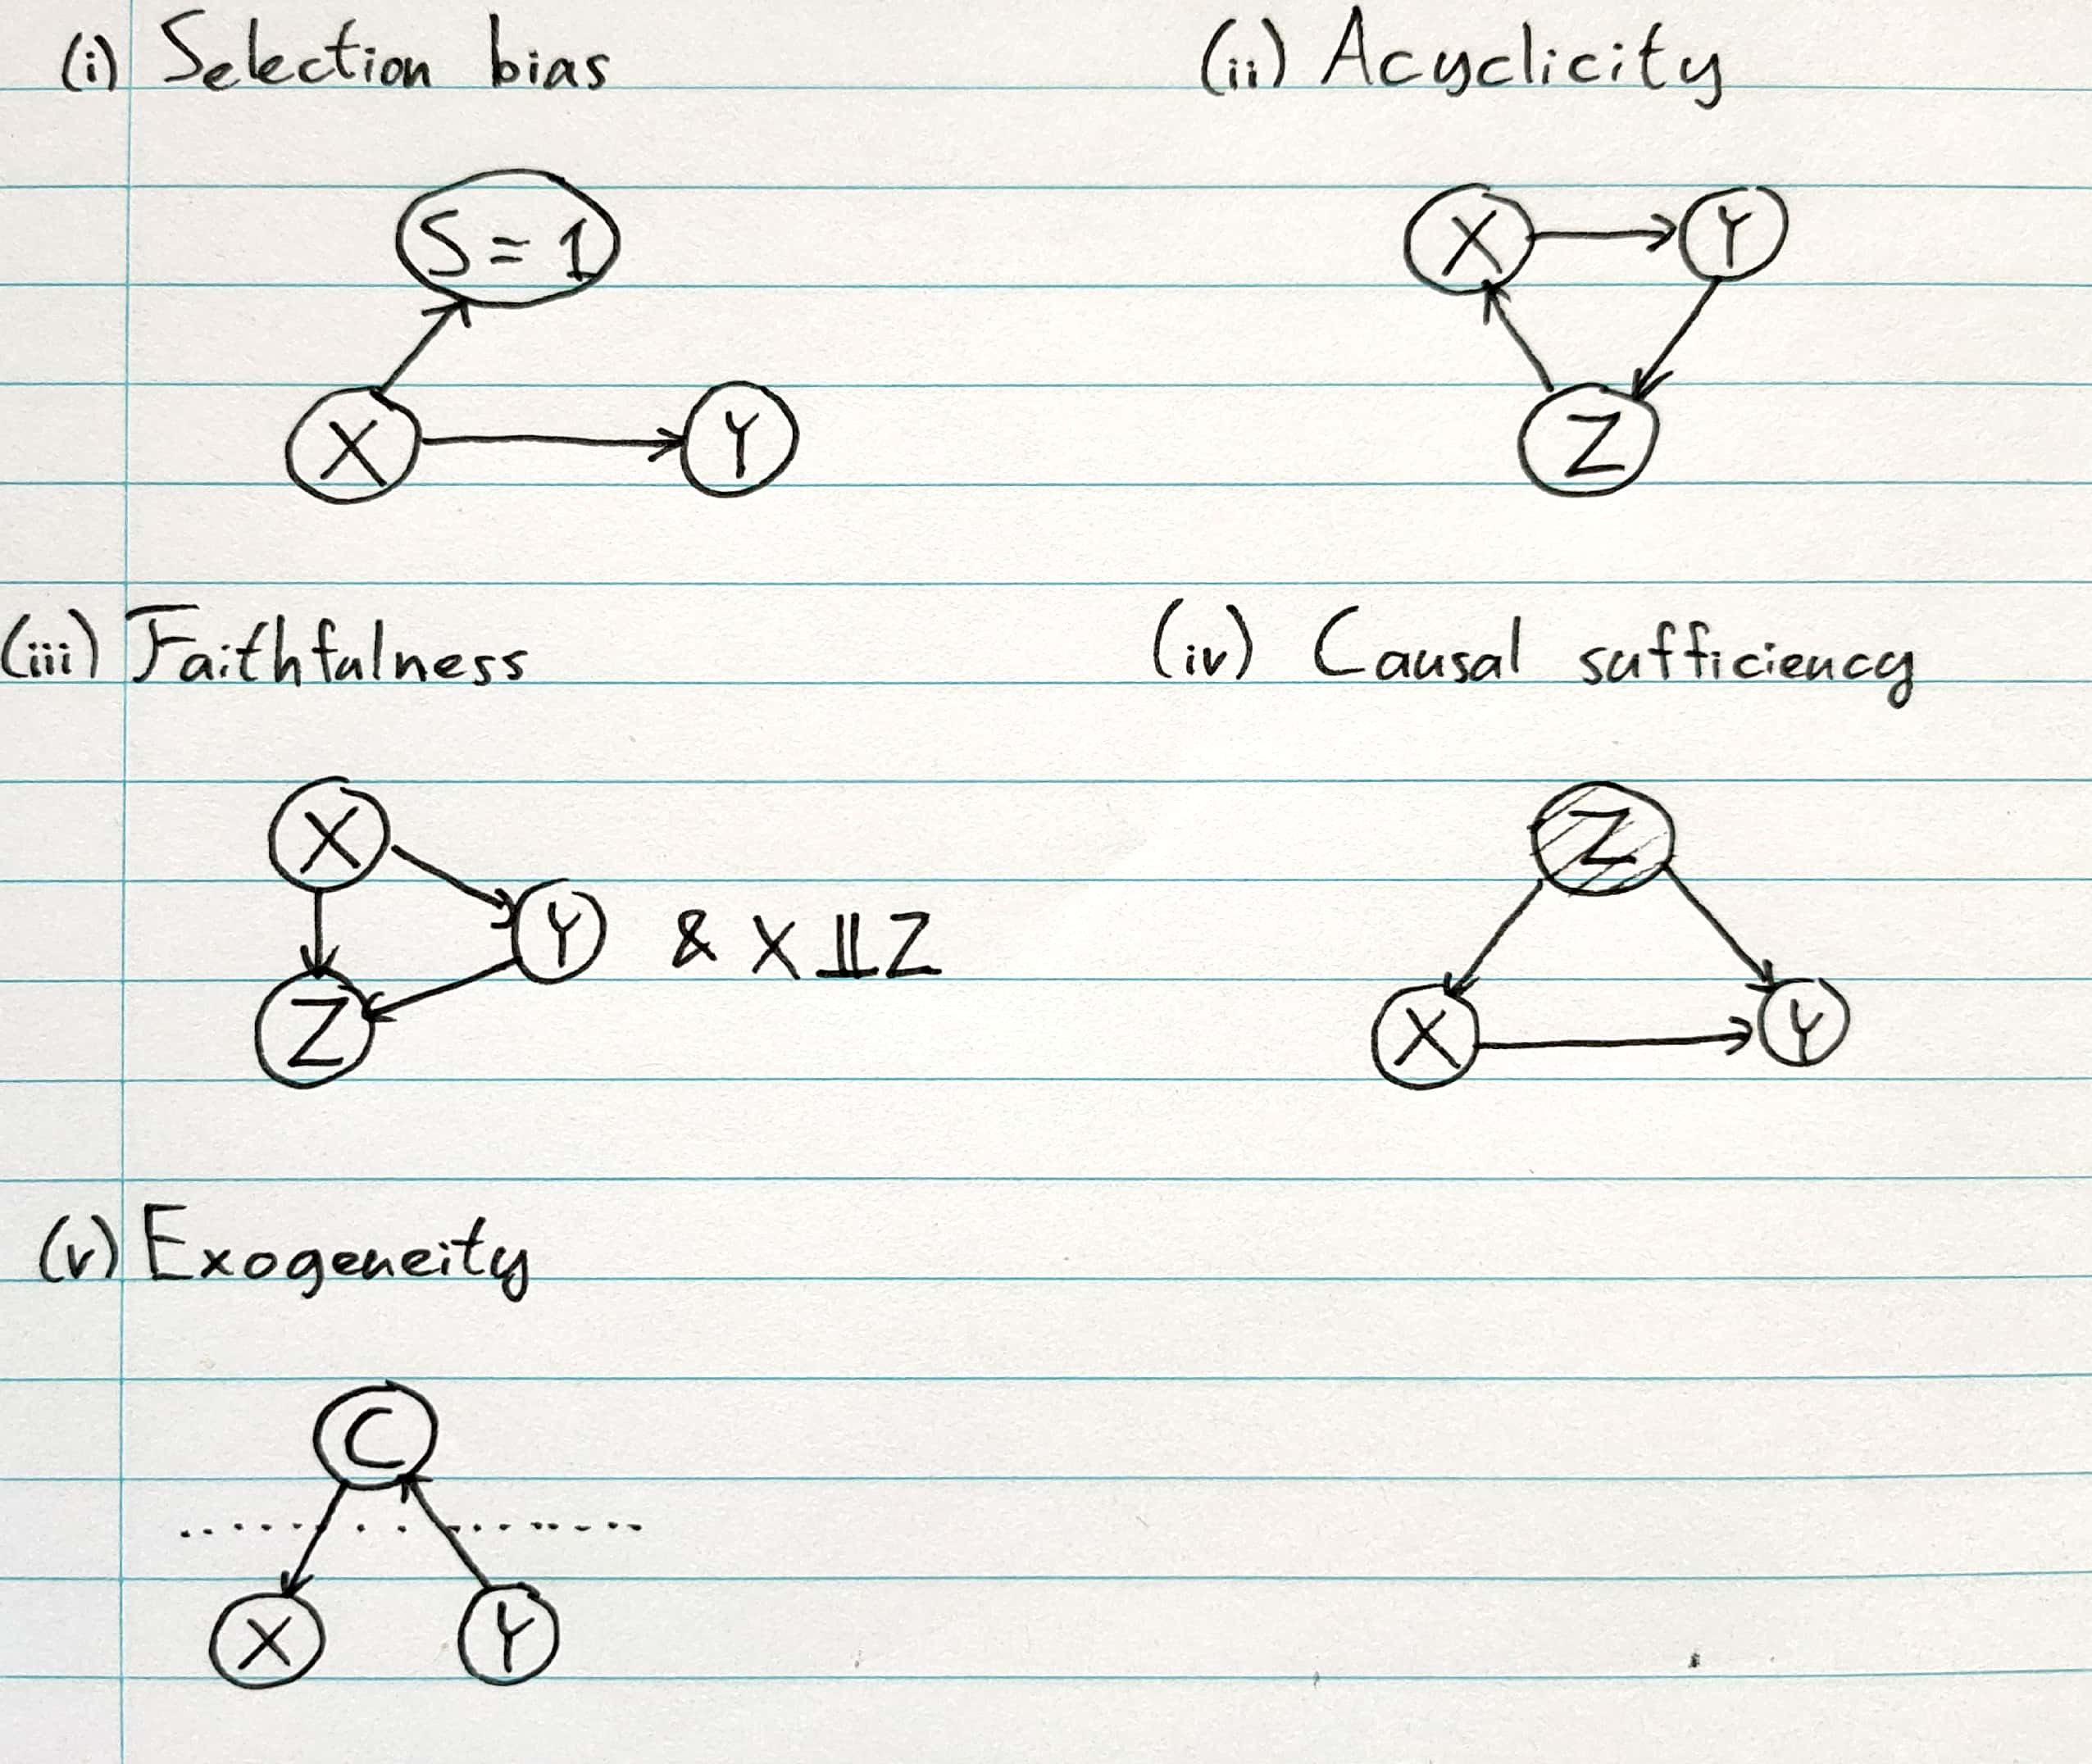
\includegraphics[width=\textwidth]{paper/2assumptions}
        \end{center}
    } 
\end{frame}


% Inspiration: Philips LCD (+ state-of-the-art)
% Aims and challenges

\begin{frame}
    \frametitle{Data and Challenges}
    
    % Data and task (my starting point was ...)
    \only<1>{
        \begin{center}
            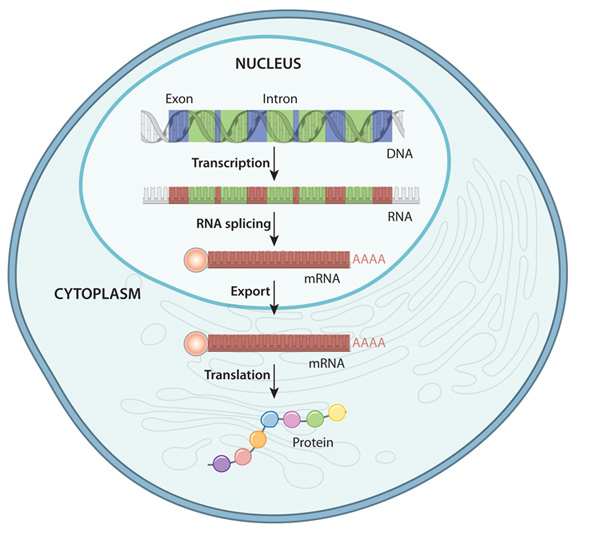
\includegraphics[height=.8\textheight]{1introduction/cell}
        \end{center}
    }
    \only<2>{
        \begin{center}
            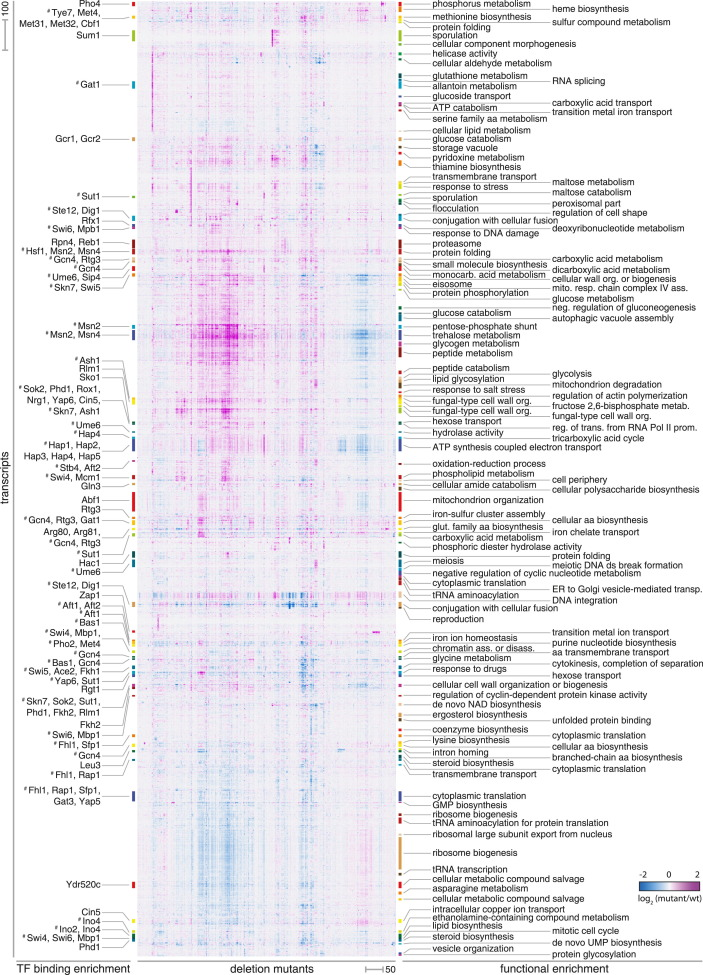
\includegraphics[height=.8\textheight]{1introduction/allinterventions.jpg}
        \end{center}
    }
    \only<3>{
        \begin{center}
            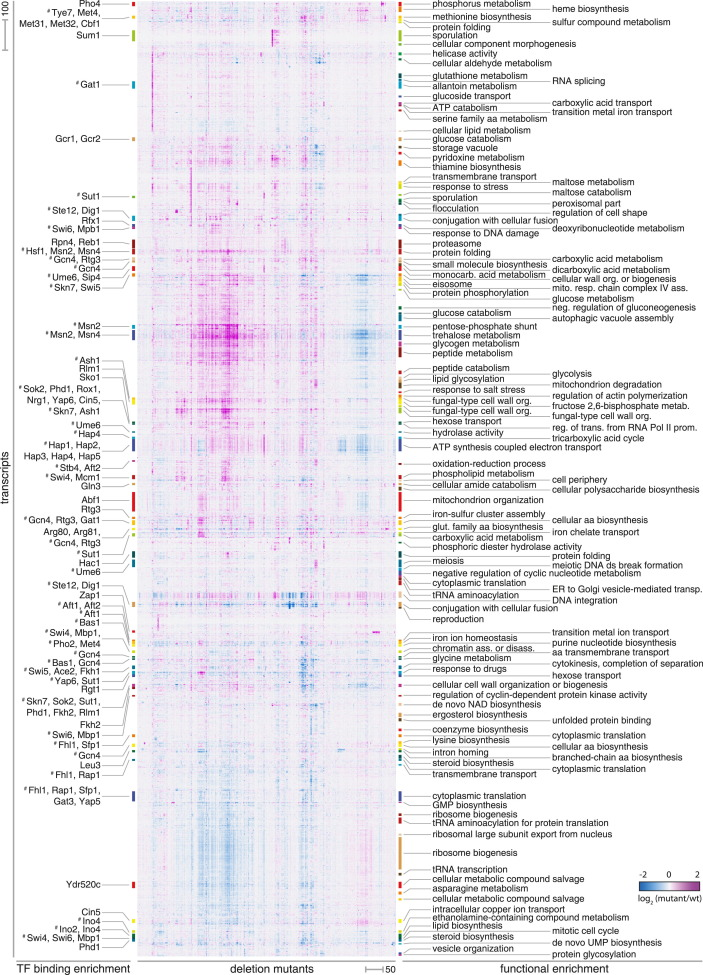
\includegraphics[width=\textwidth]{1introduction/allinterventions.jpg}
        \end{center}
    }
    \only<4>{
        \begin{center}
            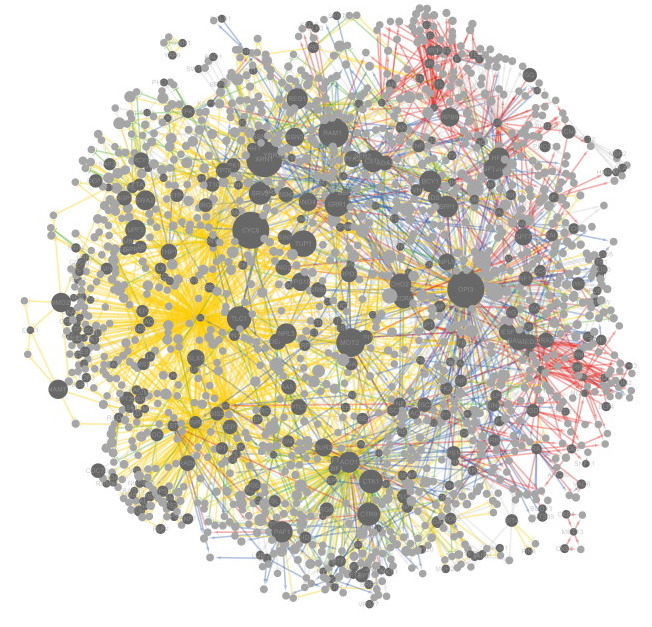
\includegraphics[height=.8\textheight]{1introduction/network.jpg}
        \end{center}
    }

    \only<5>{
        Challenges
        \begin{itemize}
            \item Sparsity
            \item High dimensionality
            \item Nontrivial evaluation
        \end{itemize}
    }

\end{frame}

% Philip and SotA
\begin{frame}
    \frametitle{Research Aims}

    \only<1>{
        \begin{center}
            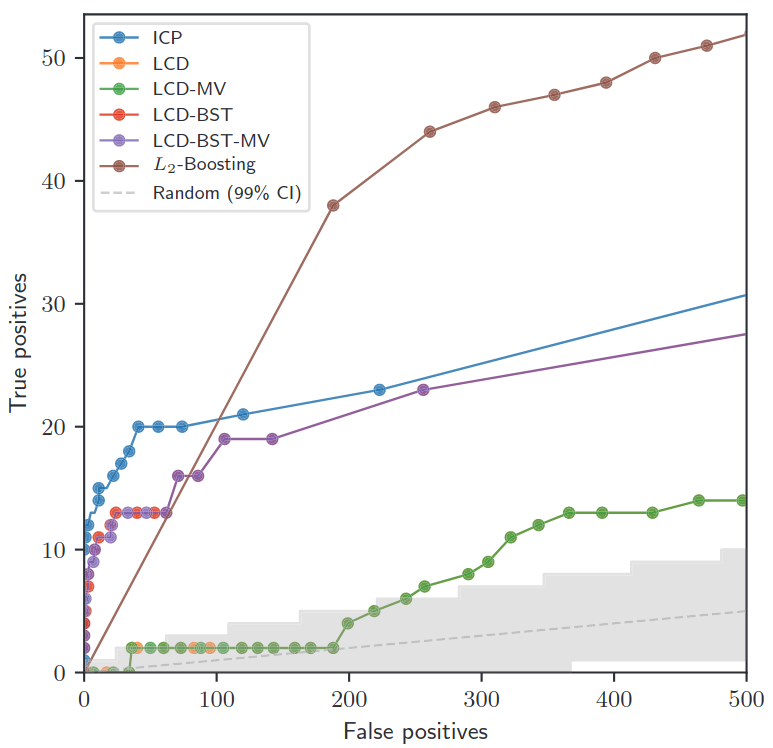
\includegraphics[height=.8\textheight]{1introduction/versteeg.png}
        \end{center}
    }

    \only<2>{
        Hypothesis:
        \begin{itemize}
            \item The \textbf{implicit order} among genes and \textbf{knowledge of intervention targets} can be used to inform the LCD method, beyond the current more crude method.
        \end{itemize}
    }

    \only<3>{
        \begin{table}[]
            \begin{tabularx}{\textwidth}{rX}
                \textbf{Research} & What properties of the dataset can be leveraged to discover causal information? \\
                \textbf{Design} & An algorithm that makes predictions based on these properties. \\
                \textbf{Research} & How is the new algorithm different from its predecessors? 
            \end{tabularx}
        \end{table}
    }
    % Aims and Challenges

\end{frame}


